
\section{Introduction}

Mass spectrometry is an important tool used to identify unknown molecular samples in a variety of applications, from characterization of organic synthesis products, to pharmacokinetic studies \cite{massspec_pharmakinetics}, to forensic studies \cite{Zhou2017LatentFingerprints},to analyzing gaseous samples on remote satellites \cite{Petrie_ions_in_space}.

In electron-ionization mass spectrometry (EI-MS), molecular samples are ionized by an electron beam and broken into fragments. The resultant ions are accelerated through a magnetic field until they reach a detector. The mass spectrum is a distribution of the frequency or intensity of each type of ion, ordered by mass-to-charge (\textit{m/z}) ratio.

A popular method for identifying a sample from its mass spectrum is to look up the spectrum in a \textit{reference library}. Here, a similarity function is used to measure the distance between the query spectrum and each spectrum in the library. If the measurement noise when obtaining the query spectrum is reasonable, then the library spectrum with the highest similarity will have the identity of the sample. A schematic of this process is shown in Figure~\ref{fig:library_matching}a.

This library matching approach is very popular, but it suffers from a \textit{coverage problem}: if the sample consists of a molecule that is not in the library, then correct identification is impossible. This is an issue in practice, since existing mass spectral reference libraries, such as the NIST/NIH/EPA MS database~\cite{2017nist}, Wiley Registry of Mass Spectral Data~\cite{mclafferty2016wiley}, and MassBank~\cite{horai2010massbank} only contain hundreds of thousands of reference spectra. The coverage problem could be reduced by recording spectra for additional molecules, but this is time consuming and expensive. For example, NIST releases updates to its library every 3 years, containing roughly 20,000 new spectra \cite{2017nist}. An alternative solution is to use \textit{de novo} methods that input a spectrum and directly generate a molecule, without using a fixed list of molecules (Section~\ref{sec:related-work}). However, these approaches currently have low-accuracy and are difficult for practitioners to incorporate into their existing work-flows. 

A third method for alleviating the coverage problem is to 
augment existing libraries with synthetic spectra that are generated by a model, instead of by an actual measurement in the lab. Thus far, this approach has not been practical, as existing spectrum prediction methods are very computationally expensive. These prediction models use quantum mechanics calculations ~\cite{bauer2016compute,grimme2013towards,Guerra_BEB_model} or machine learning~\cite{allen2016computational} to estimate the probability of each bond breaking under ionization. Since these methods must either compute molecular orbital energies with high accuracy using expensive calculations, or else stochastically simulate the fragmentation of the molecule, the time needed for each model to make a prediction scales with the size of the molecule, taking up to 10 minutes for large molecules \cite{allen2016computational}.

In response, we present Neural Electron Ionization Mass Spectrometry (NEIMS), a neural network that predicts the EI mass spectrum for a given molecule. Since our model directly predicts spectra, instead of bond breaking probabilities, it is dramatically faster than previously reported methods, making it possible to generate predictions for thousands of possible candidates in seconds. Furthermore, the approach does not rely on specific details of EI, and thus our model could be easily re-trained on mass spectra collected with alternative ionization methods.

We test the performance of our model by predicting mass spectra for small molecules from the NIST 2017 Mass Spectral Library. We find that the predictive capability of our model is similar to previously reported machine learning models, but requires much less time to make predictions. Additionally, we report the similarity of the spectra predicted by NEIMS, and further examine predicted spectra for a small set of related molecules.

\section{Related Work}
\label{sec:related-work}
Several algorithms have been developed previously for either predicting spectra or for predicting the molecule's identity given the spectrum. We review some of these techniques here.

%\begin{itemize}
\textbf{DENDRAL} One of the earliest efforts in artificial intelligence was a model used to identify molecules from their mass spectrum. Heuristic DENDRAL (Dentritic Algorithm) was a collaboration between chemists and computer scientists in the 1960s~\cite{buchanan1981dendral}. This algorithm used expert rules from chemistry to help identify patterns in the spectra and suggest possible identities for the molecule. A few years later, Meta DENDRAL was introduced to learn the expert rules that originally been given to Heuristic DENDRAL~\cite{lindsay1993dendral}.
    
\textbf{De Novo Identification Methods} Several models have been reported to predict identities of samples directly from the spectrum. Many such models have been developed for tandem mass spectrometry, where the task is to predict the original peptide sequences from digested fragments given the mass spectrum~\cite{Eng1994sequest}. Some of these methods use machine learning to achieve this task~\cite{Tran8247deepnovo, Schoenholtz2018supervision}. One work even uses machine learning models to identify personal characteristics by analyzing electrospray-ionization mass spectra of samples collected from latent human fingerprints~\cite{Zhou2017LatentFingerprints}.
    
While this approach is common for prediction of peptide sequences, it is uncommon for prediction of molecules from spectra. In recent work, a convolutional neural network (CNN) is employed to analyze the peak intensities from the spectrum and classify the molecule that made the spectrum into one of four classes\cite{spec2smiles}. The same work also attempted to employs a an LSTM sequence-to-sequence model to predict the Simplified Molecular Input Line Entry Specification (SMILES) of a molecule based on the output of the CNN~\cite{spec2smiles}. Because of the difficulty of constructing syntactically correct SMILES, this approach was not able to successfully reconstruct the entire SMILES string for any of the spectra.
    
In this work, we focus on the prediction of spectra from molecules, such that these predicted spectra can be used to improve the coverage of library-matching-based identification. The advantage of this approach over de novo approaches is that new libraries of synthetic spectra can be easily incorporated into the existing mass spectrometry software used by practitioners.
  
    
\textbf{Theoretical Calculation Prediction Methods} 
The first prediction methods for EI-MS spectrum used quantum mechanical simulation techniques to predict fragmentation events. There are three methods of predicting the mass spectrum using first principles~\cite{bauer2016compute}.
The first is to use quasi-equilibrium theory, also known as Rice-Ramsberger-Kassel-Marcus theory, to estimate the rate constants for ionization reaction~\cite{lorquet1994whither, lorquet2000landmarks, rosenstock1952absolute}.
The second is to estimate the bond order energies within a molecule, and estimate where a molecule may fragment. A related method to this second method is to calculate the cross-section of molecular orbitals upon electron impact to predict the molecule's ionization behavior~\cite{irikura2017ab, Guerra_BEB_model}.
The third method uses a combined molecular dynamics/quantum mechanics approach. The nuclei in the molecule move according to a potential energy surface for the coordinates of the molecules are determined using density functional theory. Quantum Chemistry Electron-Ionization Mass Spectrometry (QCEIMS) is a particularly recent example of the ab initio molecular dynamics method~\cite{grimme2013towards,Asgeirsson_QCEIMS,bauer2016compute}.
The trajectories resulting from this simulation are then analyzed for the presence of ionic fragments. The distribution of the ion fragments aggregated from all the simulations is then renormalized to generate a calculated EI-MS spectrum.
Each of these methods requires at least 1000 seconds per molecule \cite{allen2016computational}, and may even take days or weeks for molecules of 50 atoms. While these methods may be fast for methods involving density functional theory, they do not have the speed needed to rapidly generate a collection of spectra thousands of molecules. Some of the basis sets used for the density functional theory might not support the presence of inorganic atoms.
    
\textbf{Machine Learning Prediction Methods} Allen et al.~\cite{allen2016computational} introduced Competitive Fragmentation Modelling-Electron Ioinization (CFM-EI) to predict EI-MS spectra. This probabilistic model predicts the likelihood of breaking molecular bonds under electron ionization, and also predicts the charged fragment that is likely to form. In order to generate the spectra, it is necessary to run a stochastic simulation to determine the frequency of each molecular fragment.
In Section~\ref{sec:library-matching-results}, we directly compare this method with our proposed model.

\textbf{Similarity Metrics for Mass Spectra}

The ability to a match query spectrum from a sample to the correct spectrum in the library depends on the choice of similarity metric between spectra~\cite{mclafferty1974probability,stein1994optimization}.
A weighted cosine similarity is a similarity metric commonly used by mass spectrometry software. The exact form of the cosine similarity is given below~\cite{stein1994optimization}:

\begin{equation}\label{eq:stein-similarity}
\text{Similarity}(\boldsymbol{I}_q, \boldsymbol{I}_l) = \frac{\sum_{k=1}^{M} m_{k} I_{qk}^{0.5} \cdot m_{k} I_{lk}^{0.5}}{\left\lVert\sum_{k=1}^{M} (m_{k} I_{qk}^{0.5})^2\right\rVert \left\lVert\sum_{k=1}^{M} (m_{k} I_{lk}^{0.5})\right\rVert}
\end{equation}

where \textbf{$I_q$} and \textbf{$I_l$} are the query spectrum and the library spectrum respectively, $m_k$ and $I_k$ are the mass-to-charge ratio and intensity found at $m/z = k$, and $M$ is largest mass-to-charge ratio found in the spectra of both molecules. The reason for the weighting by $m/z$ is because the peaks in mass spectra corresponding to larger fragments are more characteristic and useful for identifying the starting molecule.

Other similarity metrics besides cosine distance similarities are also employed. For example, one other similarity method involves estimating the relative importance of one peak given the other peaks~\cite{mclafferty1974probability}. Other methods uses a Euclidian difference between peaks, or use a variation of the Hamming distance~\cite{stein1994optimization,hertz1971identification}.

In principal, machine learning could be also used to learn a parameterized similarity metric that yields improved library matching performance. However, this custom metric would be difficult to deploy, since it would require changing the software used by practitioners. 

We develop our model with the assumption that Eq.~\eqref{eq:stein-similarity} will be used for the similarity metric in downstream library matching software that consumes an augmented library.


\section{Methods}

\begin{figure}[h]
    \centering
    \begin{subfigure}{0.8\textwidth}
        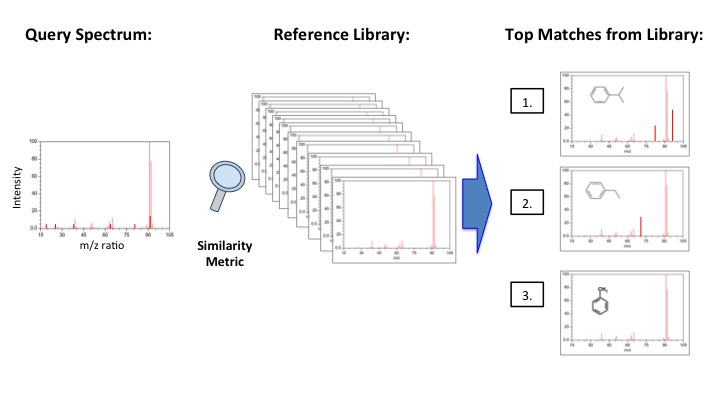
\includegraphics[width=\textwidth, trim={1cm 2.3cm 1cm 0cm}]{baseline_reference_library.jpg}
        \caption{}
    \end{subfigure}
    \begin{subfigure}{0.8\textwidth}
        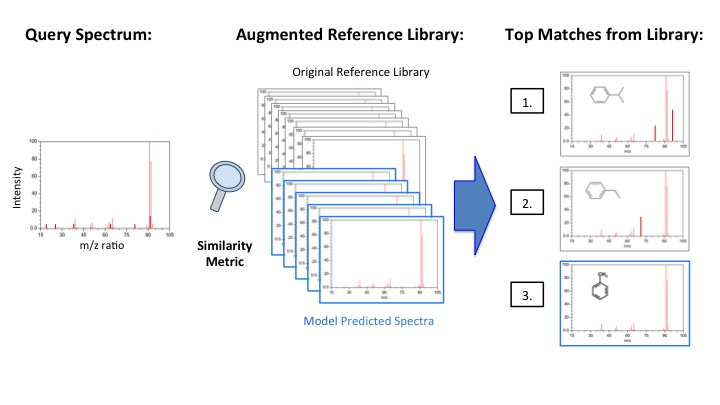
\includegraphics[width=\textwidth, trim={1cm 2.3cm 1cm 0cm}]{/Library_matching.jpg}
        \caption{}
    \end{subfigure}
    \caption{Library Matching Task. (a) A depiction of how query spectra are matched to a collection of reference spectra as performed by mass spectrometry software. (b) Query spectra are compared against a library comprised of spectra from the NIST 2017 Main Library and spectra predicted by our model.}
    \label{fig:library_matching}
\end{figure}

Our goal is to design a model that will accurately predict the EI-MS spectrum for any molecule. This will be used to produce an augmented reference library containing both predicted spectra and experimentally-measured spectra.  This task is outlined in Figure \ref{fig:library_matching}b. 

We describe our method for spectra prediction in sections \ref{sec:ms_spectral_prediction} and \ref{sec:ms_physical_phenomena}, and explain how we evaluate our model's impact on the library matching task more thoroughly in section \ref{sec:library_matching_description}.

\subsection{Spectral Prediction}\label{sec:ms_spectral_prediction}

We treat the prediction of mass spectrometry spectra as a multi-dimensional regression task. The output of our model is a vector that represents the intensity at every integral \textit{m/z} bin. We use this discretization granularity for \textit{m/z} because it is what is provided in the NIST datasets we use for training our model.

In the NEIMS model (Figure~\ref{fig:model_prediction}), we first map molecules to additive Extended Circular Fingerprints (ECFPs).  Such fingerprints record the the frequency of presence of molecular fragments, or sub-graphs within a molecule; this information is stored as a vector using a hashing function to encode the information~\cite{Rogers_2010_ECFP}. The fingerprints were generated using the RDKit Cheminformatics package~\cite{rdkit}.
These fingerprints are then passed into a multi-layer perceptron neural network (MLP). The MLP has seven layers of 2000 nodes, with residual network connections between the layers~\cite{he_resnet}. Finally, to account for some of the physical phenomena of ionization, we make some application-specific adjustments to the prediction from the MLP, described in Section~\ref{sec:ms_physical_phenomena}.

In Section~\ref{sec:library-matching-results} we compare the performance of NEIMS to that of a simple linear regression (LR) model. Here, we apply a linear transformation to the ECFP features.

To train the model, we use a modified mean-squared-error loss function. This loss funciton, shown below, follows the same weighting pattern as in Eq.~\ref{eq:stein-similarity}:

\begin{equation}\label{eq:training_loss}
    L(\boldsymbol{I}, \hat{\boldsymbol{I}}) = \sum_{k=1}^{M} m_k (I_k^{0.5} - \hat{I_k}^{0.5})
\end{equation}

where $I$ is the ground truth spectrum and $\hat{I}$ is the predicted spectrum. The intensities of the spectra were normalized after weighting by the mass and changing the power of the intensity before calculating Eq.~\eqref{eq:training_loss}. We used stochastic gradient descent to optimize the parameters of the MLP with the Adam optimizer~\cite{Kingma_adam_optimizer}.The building of the model and the optimization is done with Tensorflow~\cite{Tensorflow-2016}.

\subsection{Adjustments for Physical Phenomena}\label{sec:ms_physical_phenomena}

We make a few modifications to the MLP output to account for some of the physical phenomena of ionization in a mass spectrometer. An overview of our model is shown in Figure \ref{fig:model_prediction}. We discuss the effects of these modifications in Section~\ref{sec:library-matching-results}.

\begin{figure}[h]
    \centering
    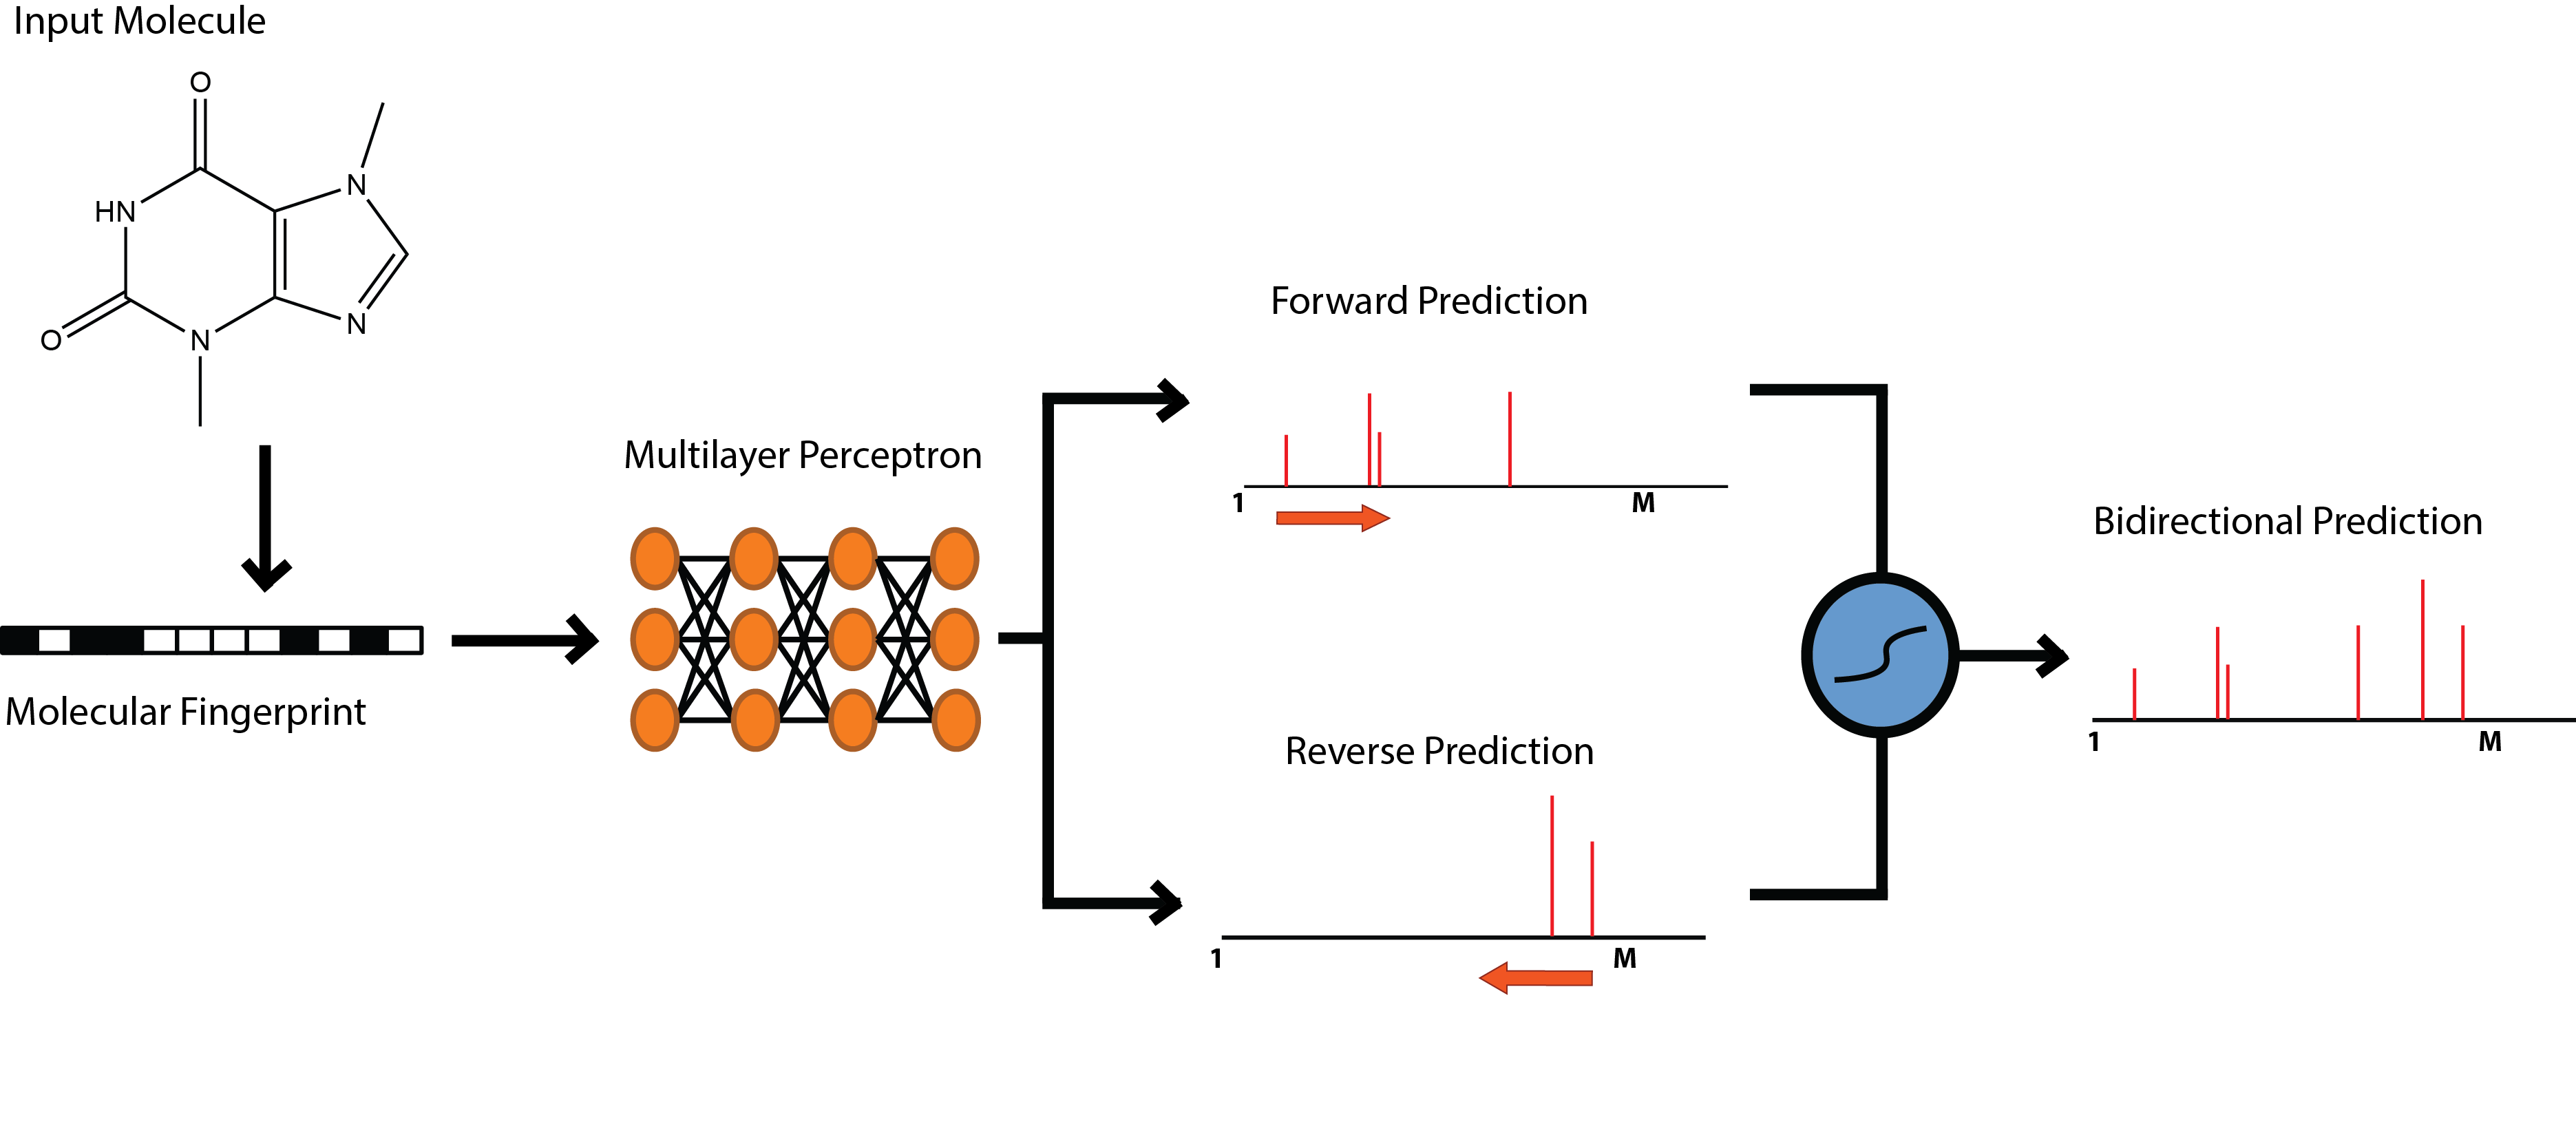
\includegraphics[width=0.8\linewidth]{Model_prediction.png}
    \caption[Neural Electron Ionization MS Prediction Model]{Molecular representations are passed into a multilayer perceptron to generate an initial output. This output is used to make a forward prediction starting at $\textit{m/z}=0$ and $\textit{m/z}=M$ and in reverse startin from $\textit{m/z}=M$ and ending at $\textit{m/z}=0$. A sigmoid gating is applied to the inputs as shown in Eq. \ref{eq:sigmoid_gate}}
    \label{fig:model_prediction}
\end{figure}

First, we zero out intensities that are located at \textit{m/z} which are greater than a few units above the molecular mass $M$. Unless the molecule contains a heavier isotope of an atom, it is not possible to have an ionization fragment that is larger than the mass of the molecule.

We also use the MLP to predict peak intensities in the \textit{reverse direction}.  The MLP described in the previous section makes predictions in the \textit{forward direction}, where the activations in the output layer of the MLP are indexed from $m/z = 1$ to $m/z = M$. We set up a layer for making predictions in the opposite direction, indexed from $m/z = M$ to $m/z = 1$. In mass spectrometry, one common fragmentation pattern is for small groups such as methyl groups ($-CH_3$, molecular weight 15Da) or chloride ($-Cl$) to fall off the main molecular ion. This event results in a peak at $m/z = M - M_k$, where $M_k$ is the mass of the fragment. Because of the wide variation in molecular mass, it is difficult for a neural network to discern this pattern by predicting only in the forward direction. However, in the reverse mode prediction, this intensity prediction will appear at index 15 for the methyl group.

Both the forward and reverse predictions are  combined to form a \textit{bi-directional} prediction. That is, the value of the MLP raw prediction at index 15 is used to contribute to the intensity both at $m/z = 15$ and $m/z = M - 15$. Instead of simply adding these two predictions, we found it useful to combine them using a coordinate-wise \textit{gate}. Here, the output layer of the MLP is of size $3M$, consisting of $M$ values each for the forward prediction, the reverse prediction, and the gate. Then, the output at position $i$ in the spectrum is given by:
\begin{equation}\label{eq:sigmoid_gate}
\sigma(\text{gate}_i) ~ \text{pred}^\text{forward}_i + (1 - \sigma(\text{gate}_i)) ~ \text{pred}^\text{reverse}_{M - i},
\end{equation}
where $\sigma(\cdot)$ is a sigmoid function.

As a final alteration, during the library match search, we have a \textit{mass filtering} option. This feature reduces the list of possible candidates in the library to only those molecules which have a molecular mass that is within some tolerance of the mass of the query molecule.
By using weak ionization methods, it is possible to identify the mass of molecule being analyzed. In some previously published models, such as the CFM-EI model, the molecular formula is used to filter the search library
~\cite{allen2016computational}. Using the molecular mass to filter the library allows more possible candidate spectra to be considered in the search.

\subsection{Library Matching Evaluation}\label{sec:library_matching_description}

We evaluate NEIMS by performing library matching using an \textit{augmented reference library} consisting of a combination of observed spectra and model-predicted spectra. We measure performance using a \textit{query set} of spectra. These spectra are from the NIST 2017 Replicates Library; this library is a collection of noisier spectra for molecules which are already contained in the NIST Main Library. The inconsistencies in these spectra reflect experimental variation, and make an informative dataset to test our model's performance.

To construct the augmented reference library, we edit the NIST Main Library, removing spectra corresponding to the query set molecules and replacing them with the predictions from NEIMS. 
We then perform library matching and calculate the similarity between each query spectrum and every spectrum from the augmented library. We record the rank of the correct spectrum, i.e. the rank of the predicted spectrum corresponding to the molecule which made the query spectrum. The similarity metric is Eq.~\eqref{eq:stein-similarity}.

For the purposes of tuning model hyperparameters, we chose to optimize recall-at-10, i.e. the fraction of our query set which achieved a matching rank of 10 or better on the library matching task. Half of the Replicates spectra were used for tuning hyperparameters, and the remaining half was evaluated for test performance. All models were trained on the spectra prediction task for 100,000 training steps with a batch size of 100.

\section{Results and Discussion}
To analyze the performance of the models, we trained with 240,942 spectra from the NIST 2017 Mass Spectral Main Library. These spectra were selected so that no molecules in the Replicates Library have spectra in the training set. When employing mass filtering, we used a tolerance of 5Da. 

\subsection{Library Matching Results}
\label{sec:library-matching-results}
\begin{figure}[h]
    \centering
    \begin{subfigure}[b]{0.52\linewidth}
        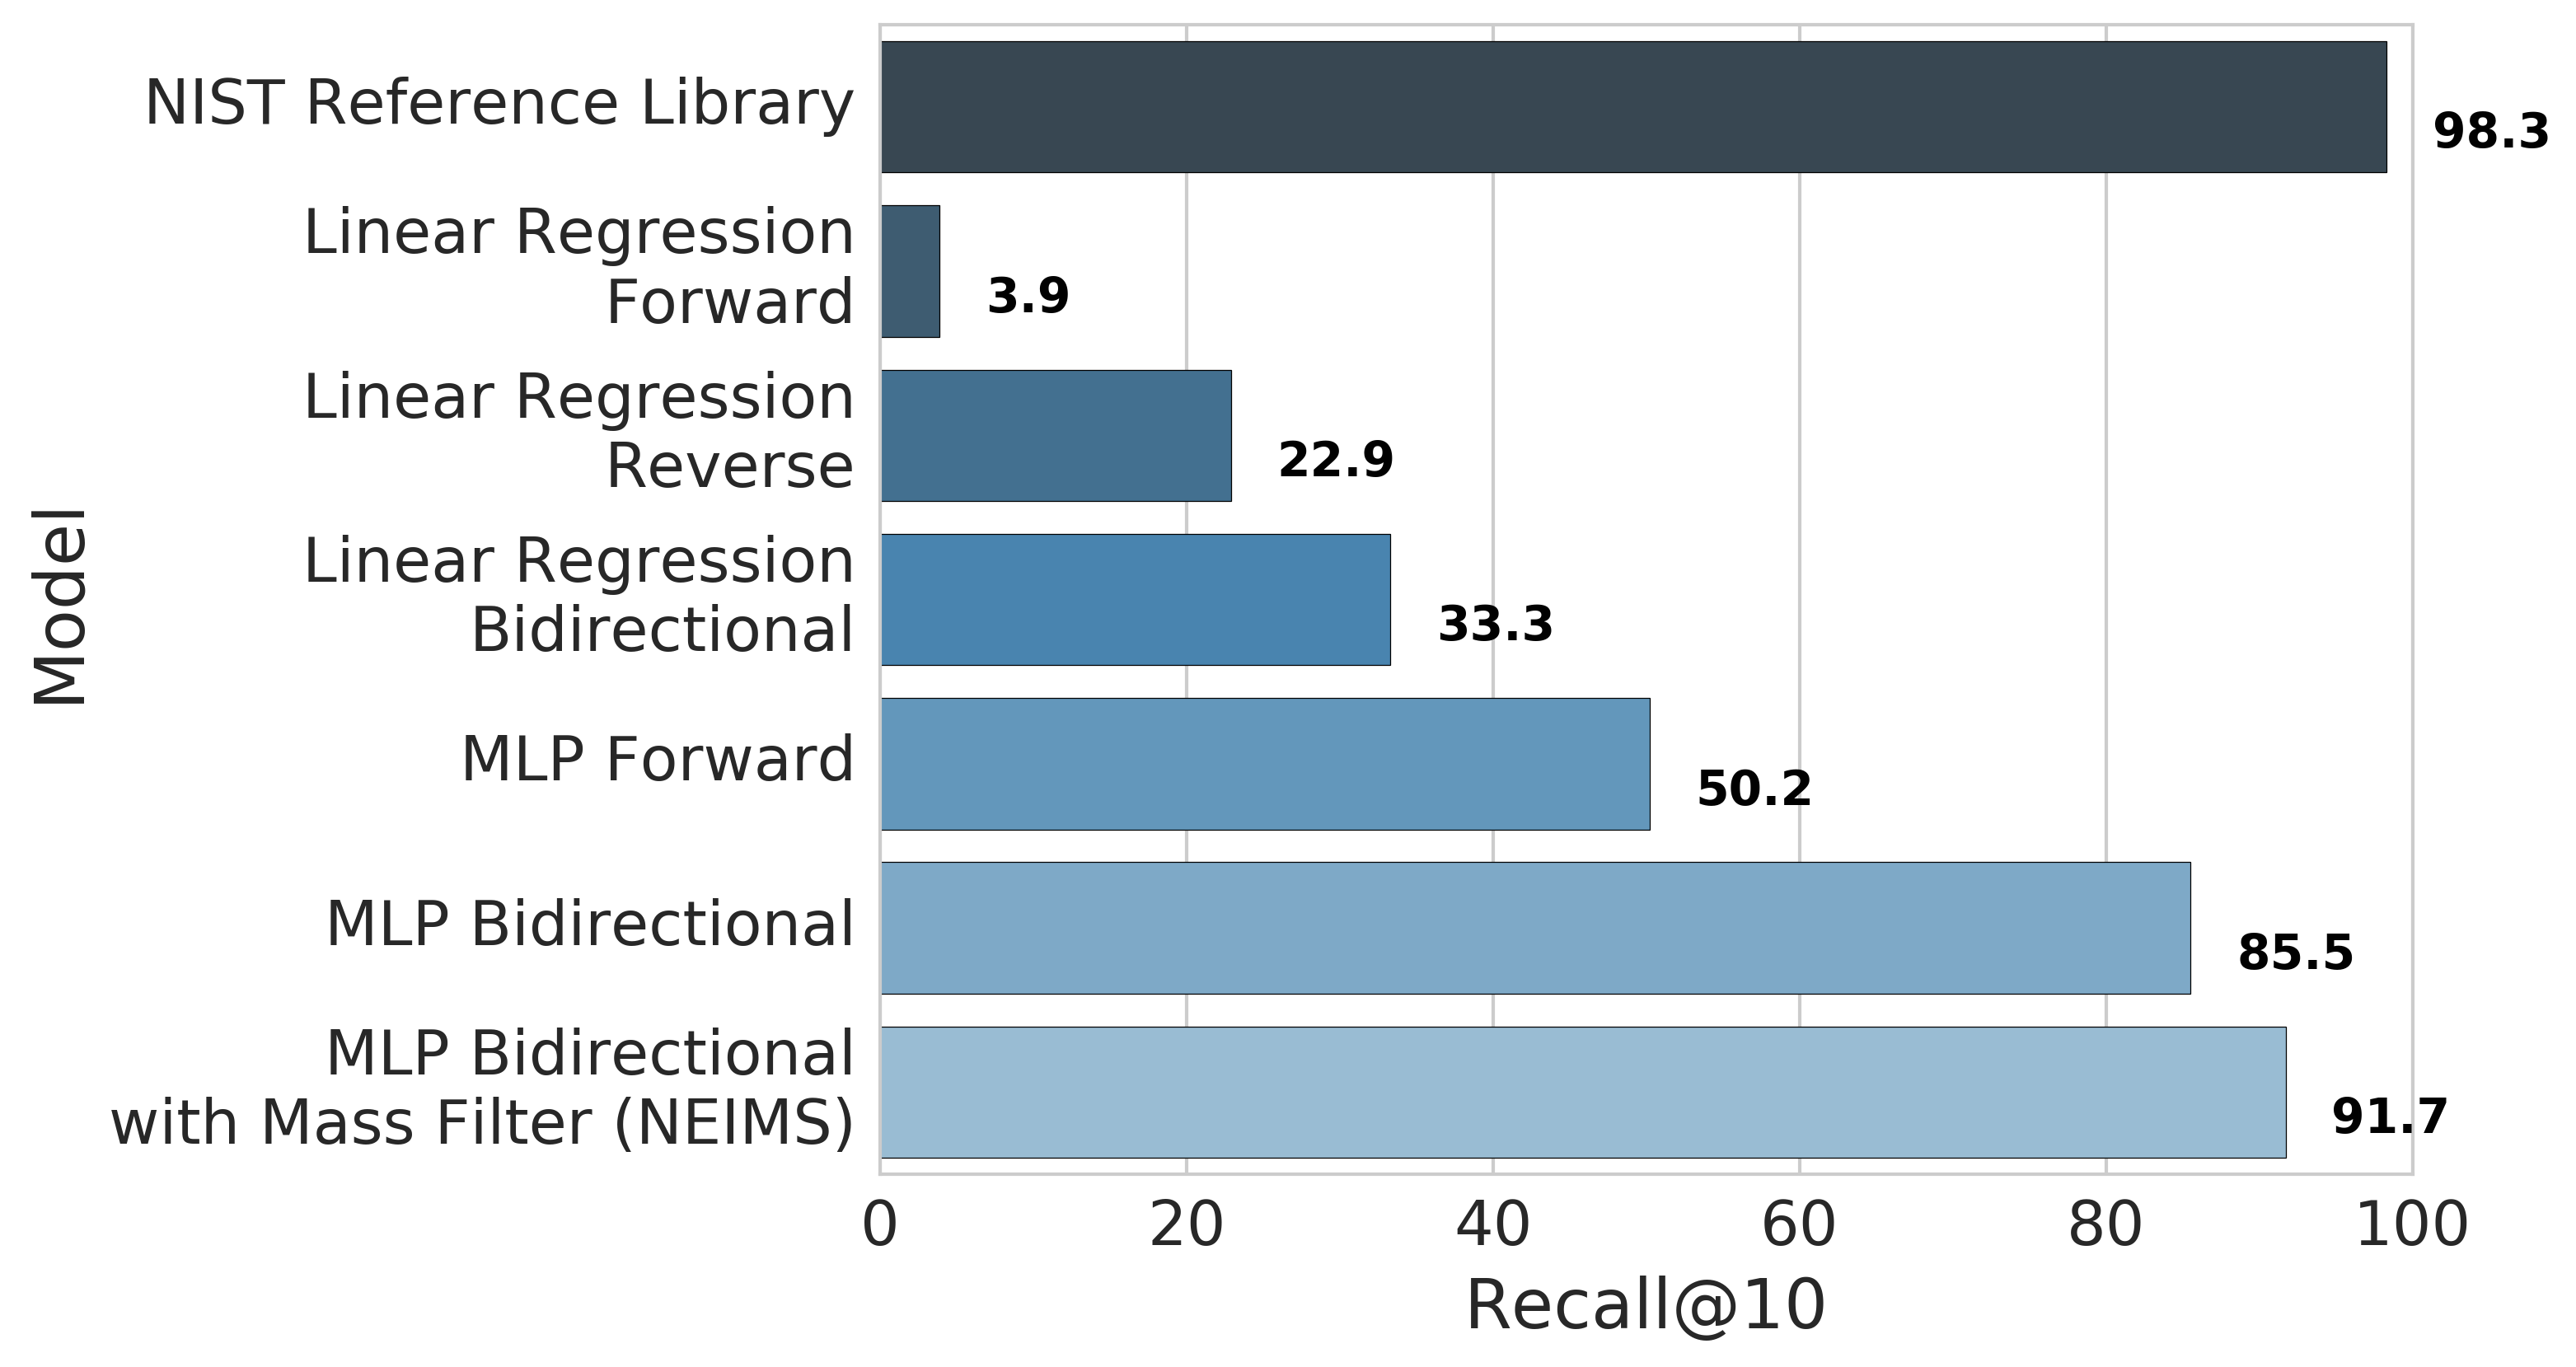
\includegraphics[width=\linewidth]{all_models_w_massfilter.png}
        \caption[Library Matching Results]{Library matching performance on different models}
    \end{subfigure}
    \begin{subfigure}[b]{0.4\linewidth}
        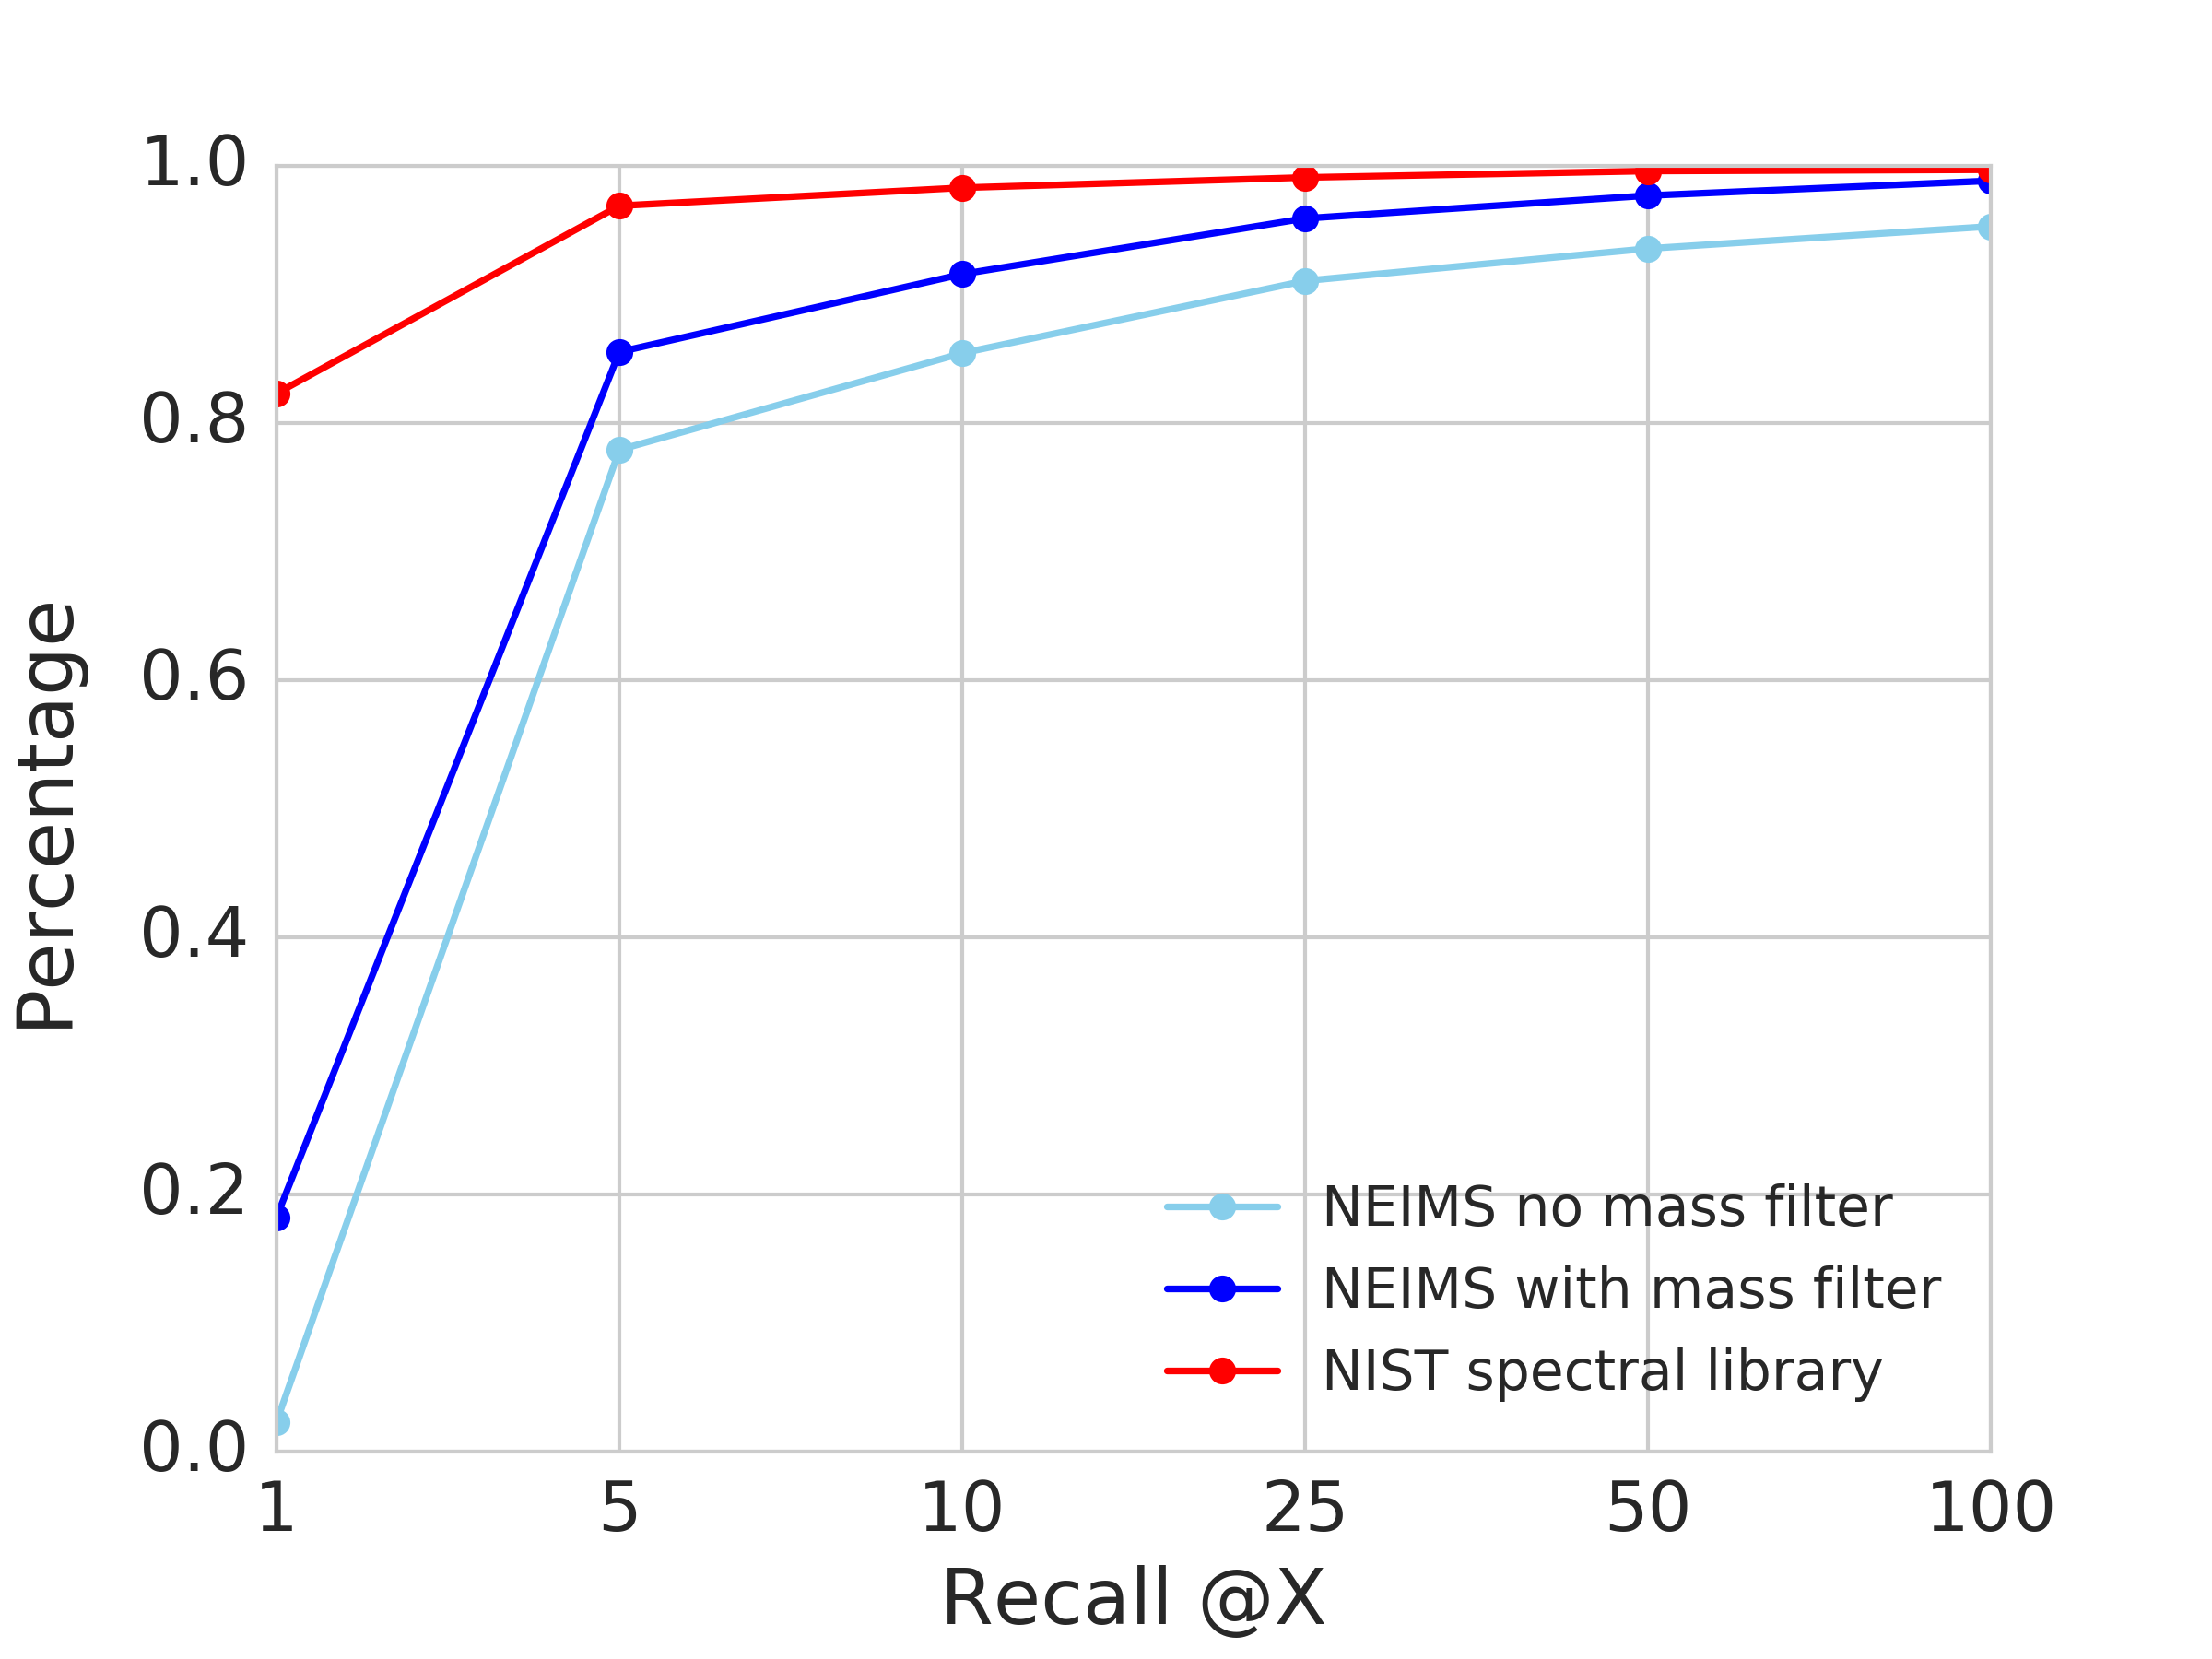
\includegraphics[width=\linewidth]{recall_at_X.png}
        \caption[Recall@X Results for Different models]{Recall Results at various levels}
    \end{subfigure}
    \caption{Performance of different model architectures.}
    \label{fig:main_results_and_recall_results}
\end{figure}

We first examine the effect of our various modeling decisions on performance. Figure \ref{fig:main_results_and_recall_results}a compares the performance of forward, reverse, and bidirectional versions of the linear regression and MLP models on the library matching task. 

The top row of Figure \ref{fig:main_results_and_recall_results} shows that it is not possible to achieve perfect recall accuracy on the library matching task even when using the NIST reference library itself, and no predicted spectra are included.
It achieves 86\% recall@1, and 98.3\% recall@10. This serves as a practical upper bound on achievable library matching accuracy and reflects the experimental inconsistencies between between the main library spectra and replicates spectra. These inconsistencies are due to the general variability of the mass spectroemtry measurement noise. 

The forward prediction mode for both the linear regression model and the multi-layer perceptron (MLP) has poor performance. The library matching performance for the linear regression model is improved by ~20\% when switching to using  reverse mode prediction. Using  bi-directional prediction mode improves  recall@10 accuracy by 30\% for both the linear regression and the multilayer perceptron model. This finding suggests that the bi-directional prediction mode is more effective at capturing the fragmentation events than the forward-only model.

Figure \ref{fig:MLP_improvement_spectra} shows the improvement in spectral prediction for pentachloro-benzene. Note that the bidirectional model on the left more accurately models the larger \textit{m/z}. The intensity peaks for larger \textit{m/z} are critical for determining the identity of a molecule, and are more heavily weighted in the library match similarity function.

\begin{figure}[h]
    \centering
    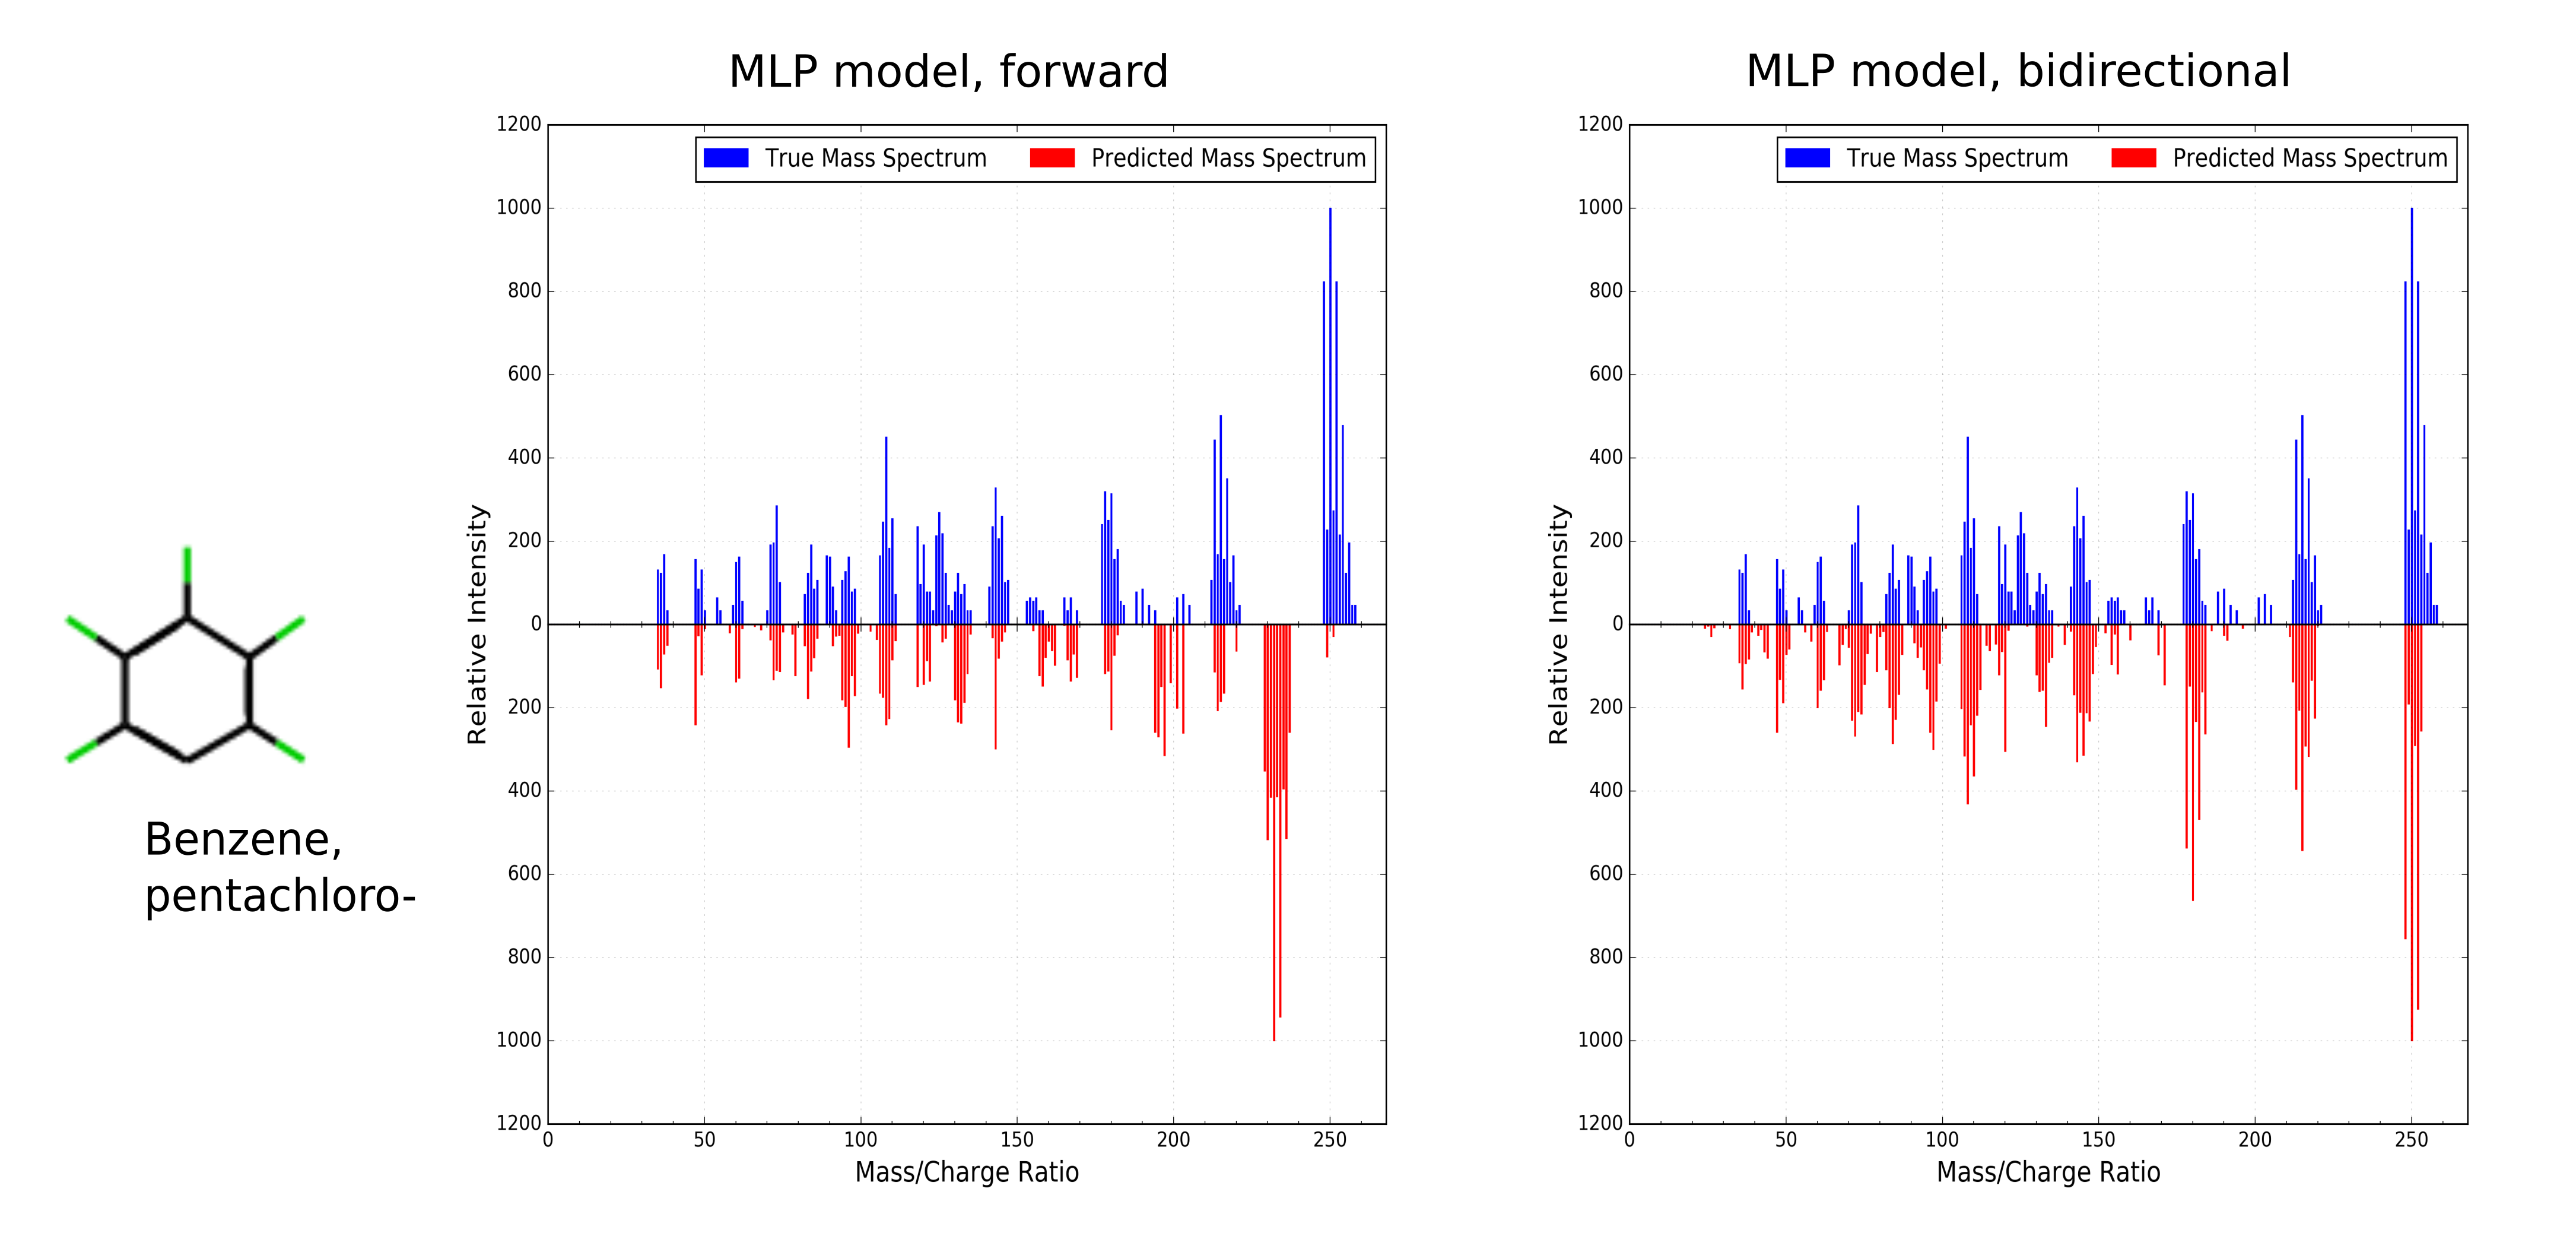
\includegraphics[width=0.8\linewidth]{CEOCDNVZRAIOQZ-UHFFFAOYSA-N_mlp_model_spectra.png}
        \caption[Sample Spectra Prediction]{Spectral Prediction with MLP forward Model (left) and MLP bidirectional Model (right). The true spectra is shown on the top, while the predicted spectra is shown inverted below.\footnotemark Note that the spectrum predicted by the bidirectional model shows fewer stray peaks than the forward model, particularly at the right hand side of the spectrum, which the reverse prediction is designed to capture.}
    \label{fig:MLP_improvement_spectra}
\end{figure}

\footnotetext{Images for spectral prediction results are inspired by the spectral prediction images in Bauer et al.\cite{bauer2016compute}}

NEIMS achieves 91.7\% recall@10 After applying a mass filter. The mass filter was set to a tolerance of 5 Daltons of the query molecule's mass; this reduces the size of the library to a median of 6,696 spectra for each query molecule. 
For the rest of this report, we will refer to the bi-directional multi-layer perceptron model with mass filtering as the default settings for NEIMS.

From Figure \ref{fig:main_results_and_recall_results}b) we see that NEIMS while NEIMS has comparable performance for recall levels of 10 and above, it has considerably worse performance for Recall values of 1 and 5. This result is unsurprising given that the hyperparmaters of the model were trained to maximize performance on Recall@10. If Recall@1 was selected to tune the hyperparameters, the performance accuracy would likely improve, however this model becomes much more difficult to train due to the small amount of signal when the model begins to train.

\subsection{Performance on NIST'14 dataset}
\label{sec:NIST14-results}

We next compared our model's performance directly to the performance of the CFM-EI model~\cite{allen2016computational}. The setup of Allen et al. differs from our current setup in two ways. First, they evaluate their model on the NIST 14 spectral library. Second, while they also use the Replicates Library for their query set, their augmented spectra library contains only spectra predicted by their model, and none from the original library. Third, the similarity metric used for evaluation in library matching in CFM-EI uses a slightly different weighting requirement \eqref{eq:stein-similarity}. In CFM-EI, the cosine similarity is weighted $m_k^{0.5}$ instead of $m_k$ so the larger peaks receive less importance~\cite{allen2016computational}.
We retrain our NEIMS model on the NIST 14 dataset, and evaluate the performance using the NIST 14 replicates as the query set. We match their setup identically, incorporating only predicted spectra into our augmented library, and using the same modified similarity metric.

\begin{table}[h]
    \centering
    \begin{tabular}{c|c|c|c}
        Model & Recall@1 & Recall@10 (\%) &  Average run time (ms) \\
        \hline
        NIST '14 Reference Library & 77 & 98.7* & -- \\
        CFM-EI & 42.6 & 89* &  300,000 \\
        NEIMS & 54.3 & 92.7 &  0.47ms
    \end{tabular}
    \caption{Performance on Library matching task for NIST 17. * indicates that values were estimated from  Figure 4 of Allen et al.~\cite{allen2016computational}}
    \label{tab:NIST14_results}
\end{table}

The library matching performance for CFM-EI and NEIMS are compared against the NIST14 library for library matching performance are reported in Table\ref{tab:NIST14_results}. NEIMS performs slightly better than CFM-EI on the library matching task. 

In terms of timing, NEIMS is able to make spectral predictions much more quickly. With NEIMS, it would be possible to generate spectra for 1 million molecules in 90 min on a CPU, with potential for speedup with a GPU. 


\subsection{Spectral distance and its effect on performance}

\begin{figure}[h]
    \centering
    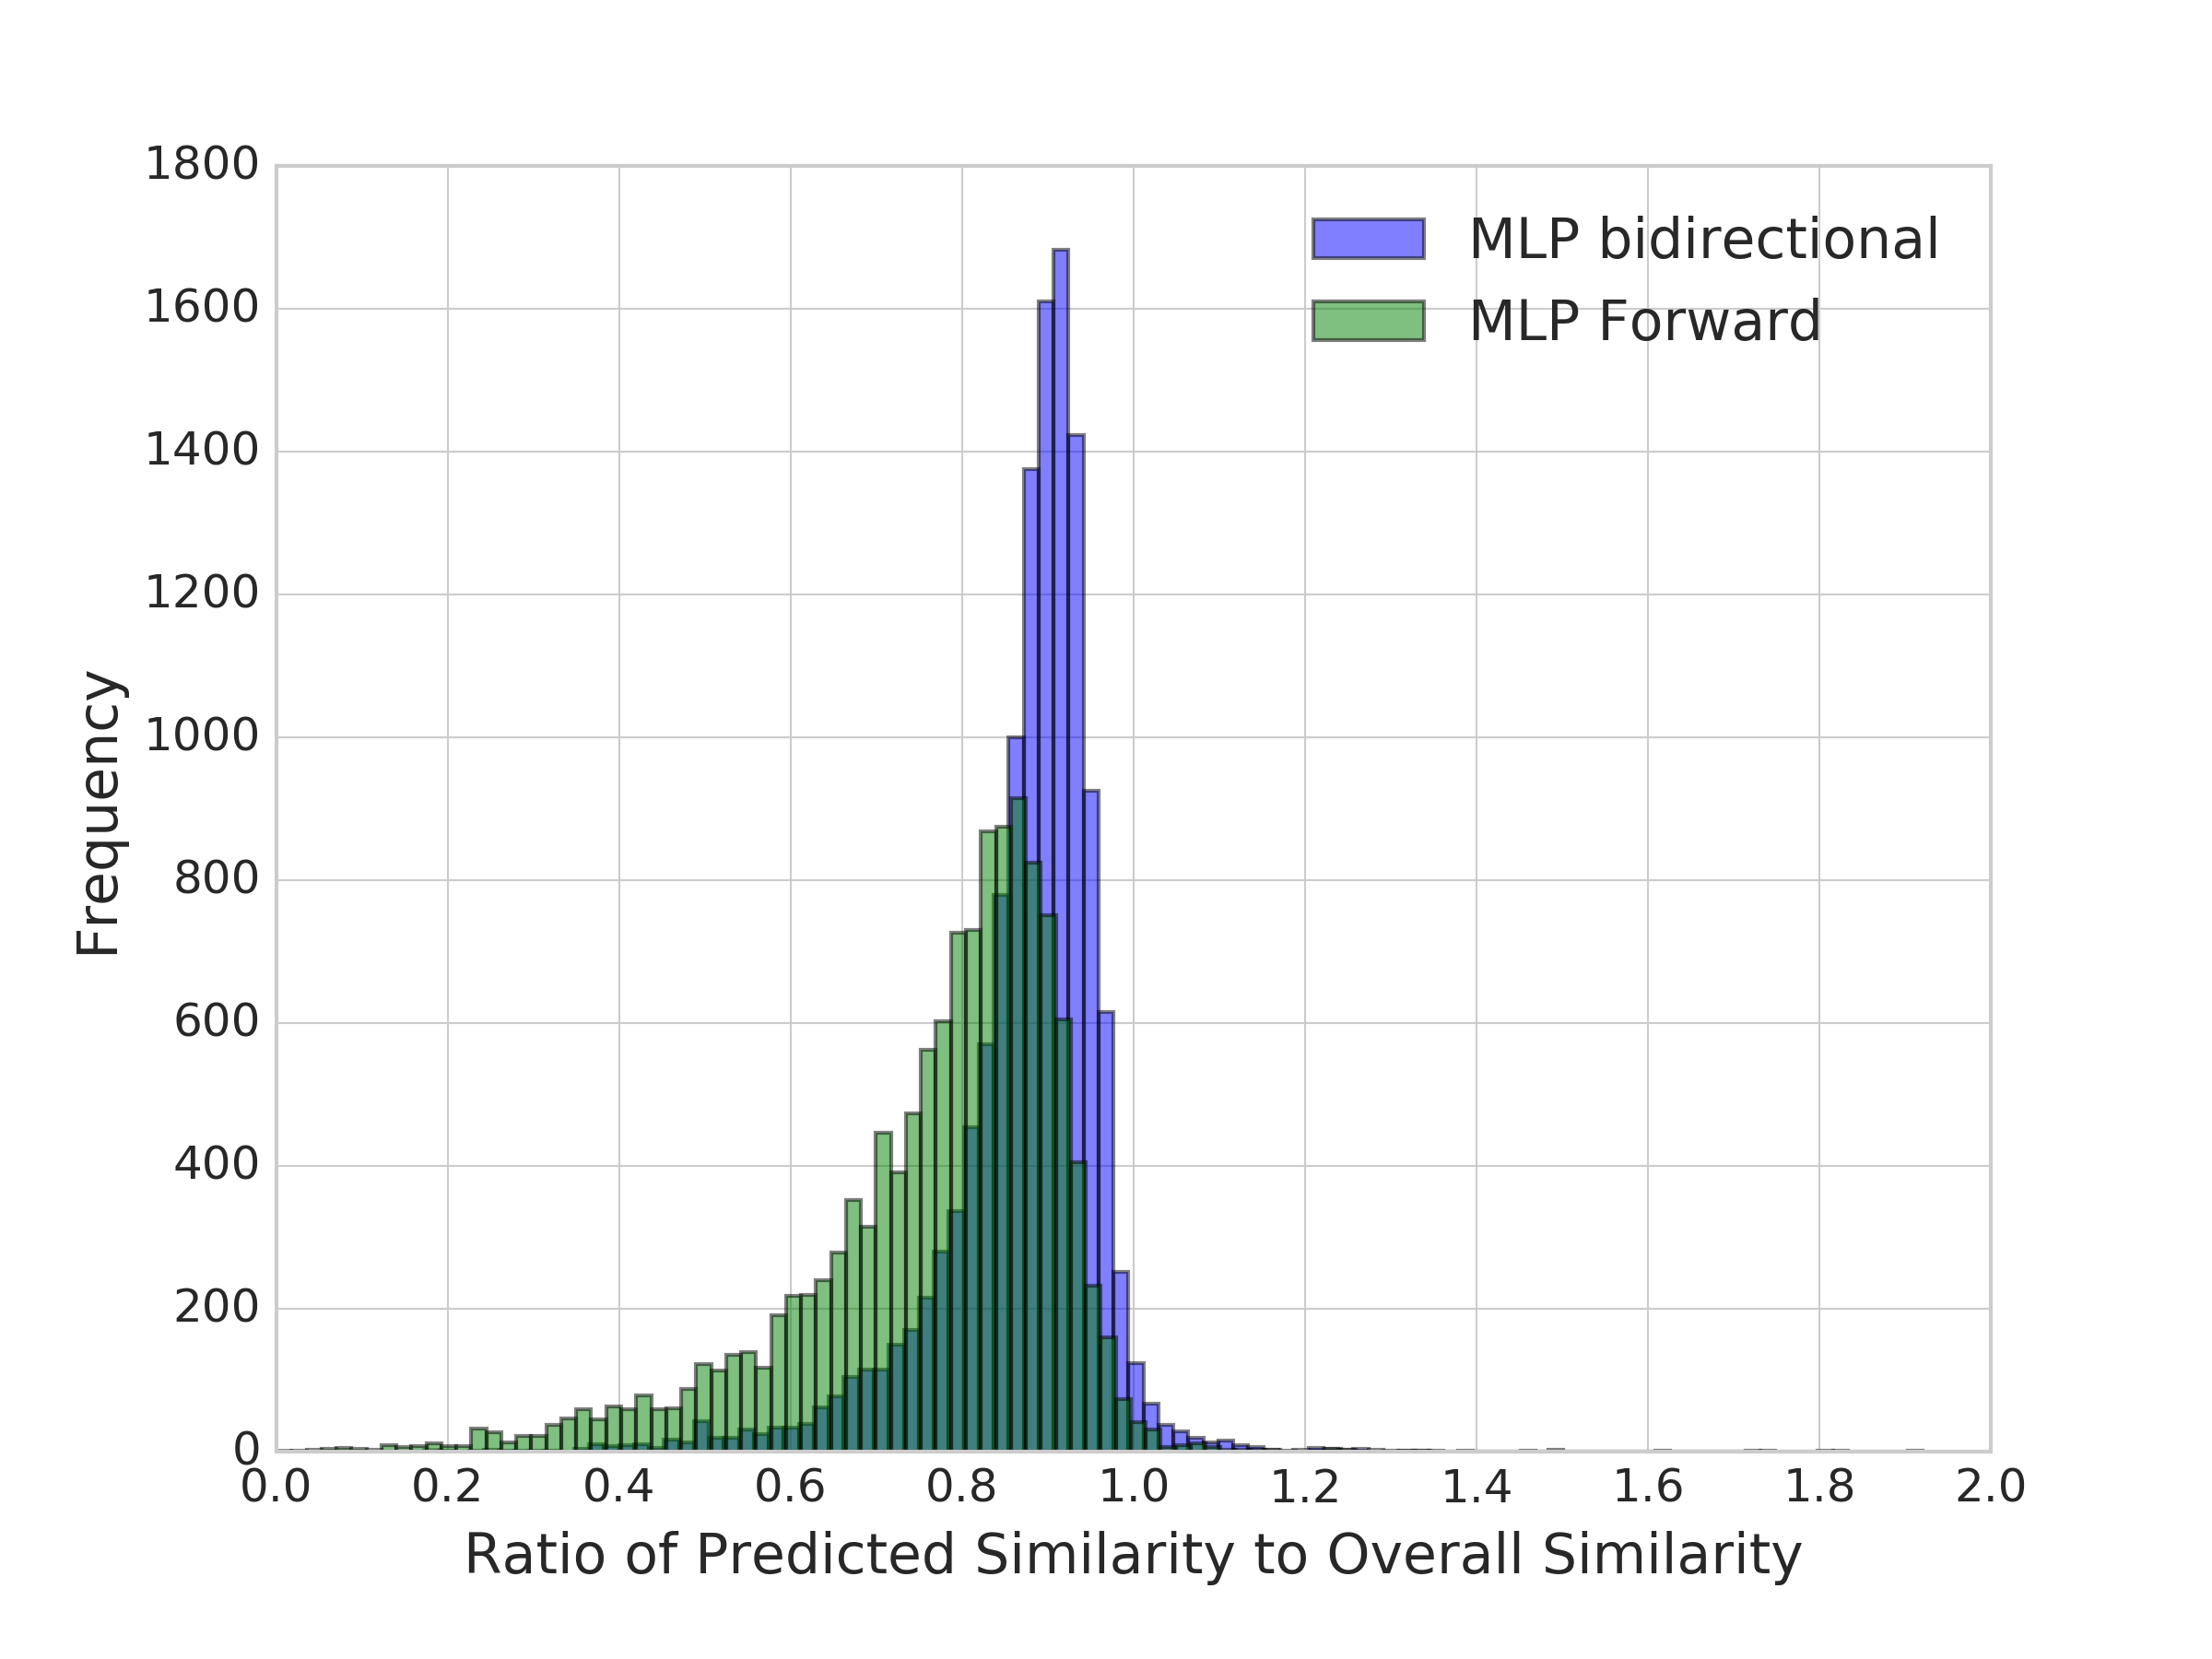
\includegraphics[scale=0.4]{predicted_similarity_overall_similarity_ratio.png}
        \caption[Similarity Analysis of NEIMS predicted spectra to spectra self-similarity]{Comparing the similiarity between the predicted spectrum and the ground truth spectrum to the overall similarity between spectra for the same molecule. }
    \label{fig:similarity_analysis}
\end{figure}

In order to observe the quality of spectral predictions from NEIMS individually rather than in aggregate from library matching performance, we observe the similarity between the predicted spectra and the training spectra.

We measure similarity between spectra using the weighted cosine distance in Eq. \ref{eq:Stein-similarity}; we refer to this similarity as the \textit{predicted similarity}.

Because of the noise inherent in mass spectra measurements, it is important to contextualize the predicted similarity against the self-similarity of recorded spectra for a given molecule. We measure the similiraty between spectra for each molecule in the query set, and refer to this as the \textit{overall similarity}.

By observing the predicted similarity to overall similarity ratio we can make judgments about the quality of NEIMS predictions for a given molecule in the context of the amount of intrinsic noise for that molecule.
Figure \ref{fig:similarity_analysis} shows that for the MLP bidirectional model, roughly half of the spectra have a predicted similarity to overall similarity ratio that is greater than 0.9. Some of these molecules even have ratios that are greater than 1, indicating a particularly low overall similarity. This indicates that the predicted spectra do not differ much more significantly from the ground truth spectra than the replicates.
It is also apparent that the bidirectional MLP model has a much higher ratio than the forward MLP model, indicating better spectra prediction. 

\subsection{Bit Analysis of Input Fingerprints}

In order to understand what mass spectrometry fragmentation patterns NEIMS might have identified from the training process, we analyze the performance of the model based on the frequency of presence of bits from the 4096-bit ECFP fingerprint with radius 2 which represents the molecule.

These groups of molecules were identified as follows: First, molecules from the query set were sorted according to their library matching accuracy. Molecules whose query spectra had a perfect match, i.e. molecules which were correctly identified in the library matching process, were selected as the group of high-performing molecules; there were 5429 such molecules. Conversely, molecules whose query spectrum were matched at a rank of 50 or higher in the library matching task were designated as the low performing set; this set comprised of 827 molecules. This analysis was done with using many useful tools from this RDKit blogpost~\cite{rdkit_blogpost_bit_statistics}.

Next, we measure the frequency of every ECFP bit within each set, and compare that the frequency of each bit in the entire NIST 17 main library. For the high-performing molecules, we focus on those bits which occur disproportionately often, namely which are 4-6 times more frequent in the query set than in the library. Because the molecular fragments corresponding to these bits are less common in the library, NEIMS would need to identify fragmentation patterns on fewer training examples. For the low performing molecules, we focus on those molecules whose bits are expressed more frequently, ~10 times more frequently, in the training set than in the test set. This suggests that despite having many examples of molecules with this bit turned on, NEIMS was unable to identify a pattern to use in reconstructing spectra.

\begin{figure}[h]
    \centering
    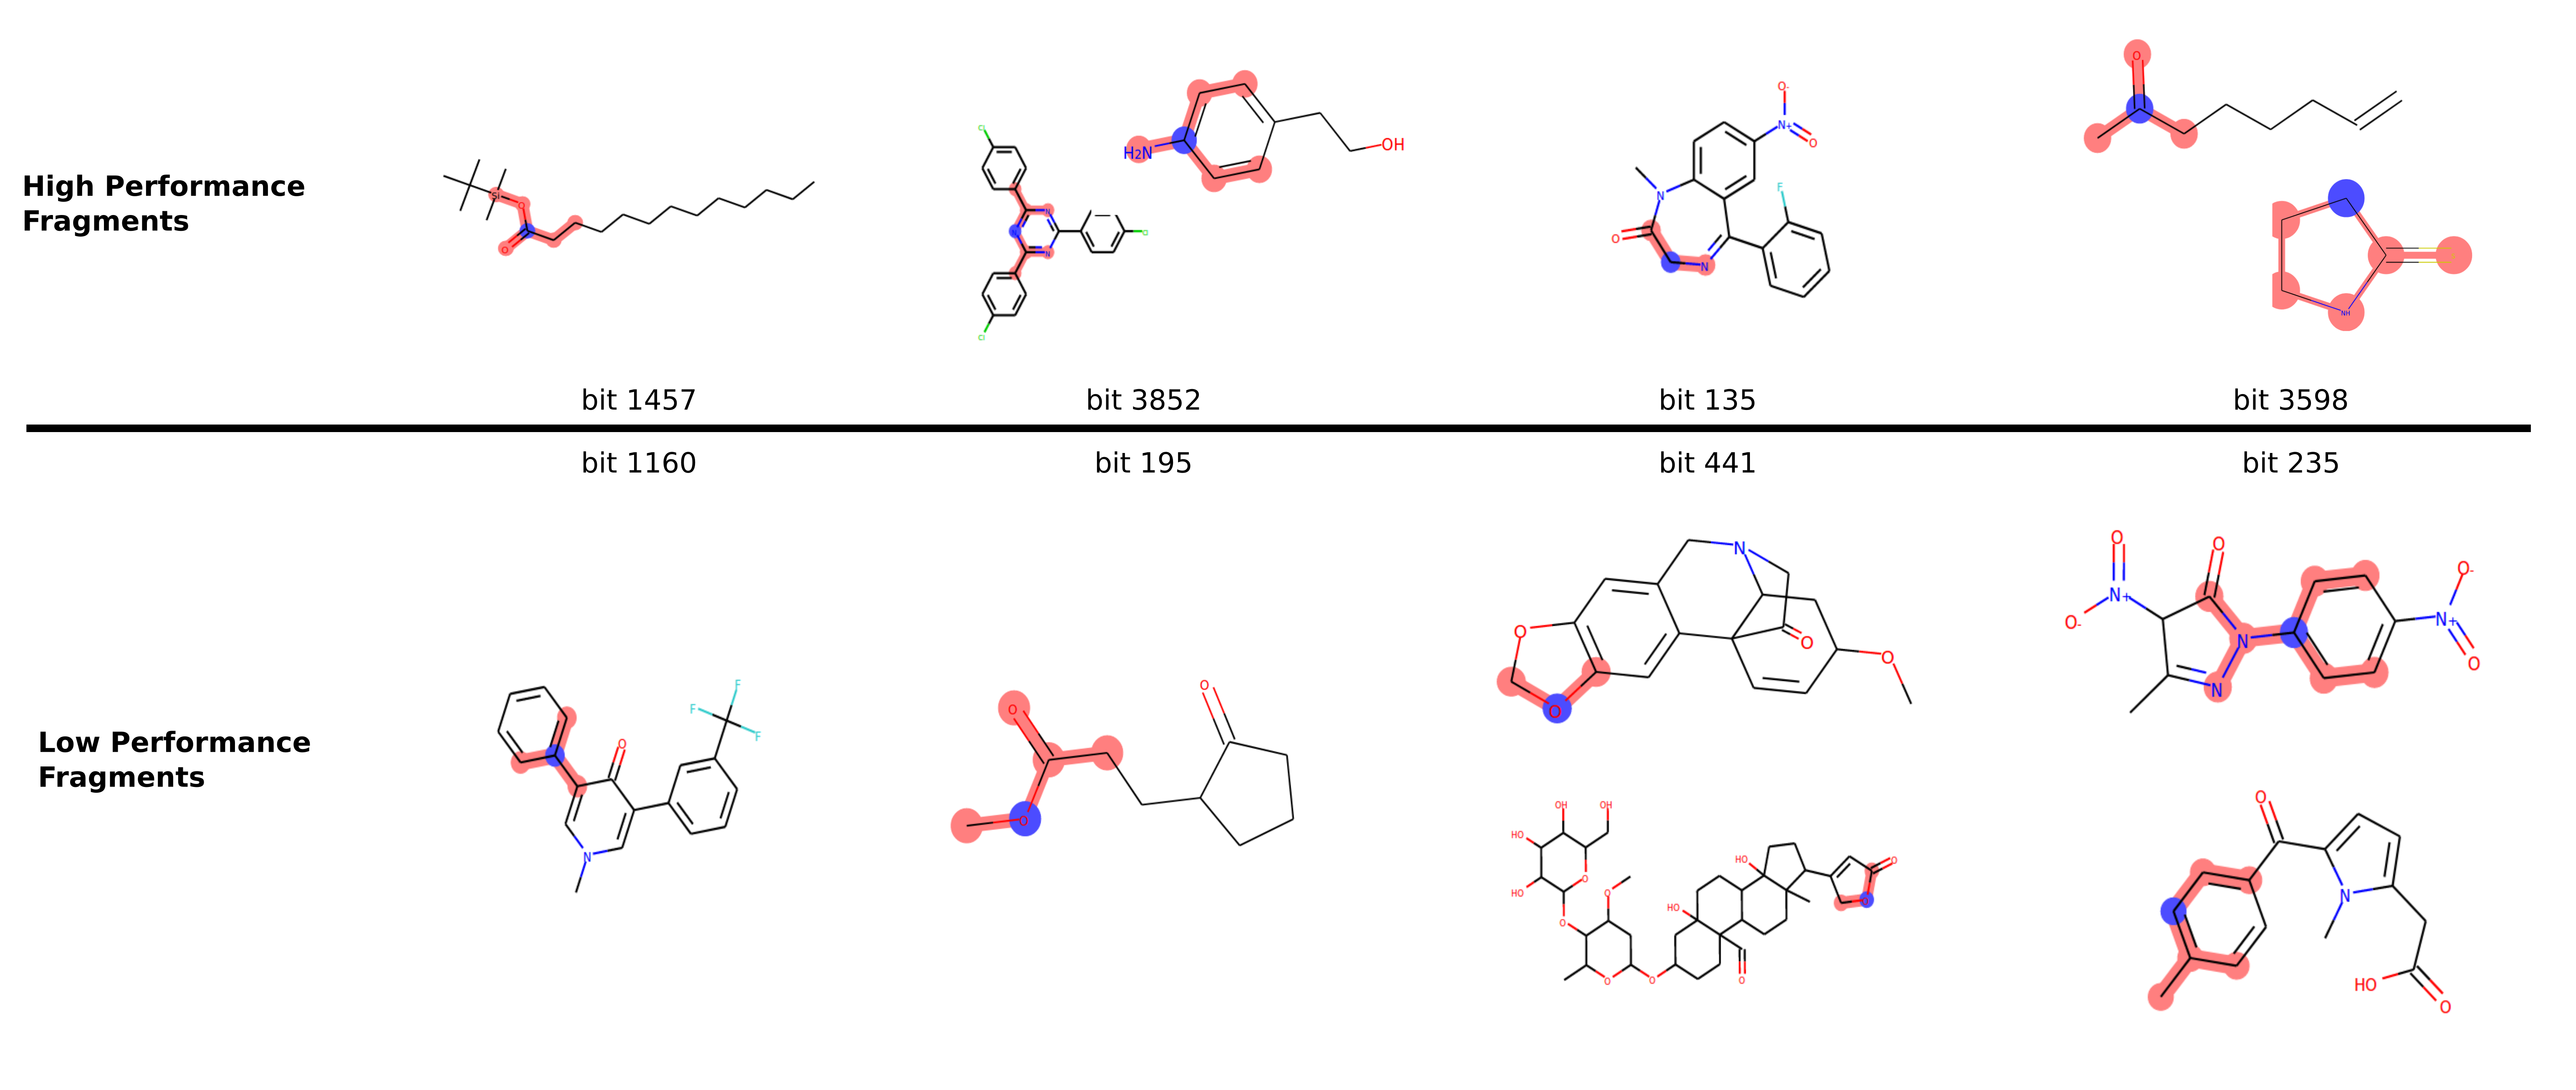
\includegraphics[width=0.9\linewidth]{good_bad_molecules_horiz.png}
        \caption[Sample Selection of Fingerprint Bits with High and Low Predictive Accuracy]{A selection of molecule fragments corresponding to bits with high and low performance.}
    \label{fig:good_bad_bit_figures}
\end{figure}

Figure \ref{fig:good_bad_bit_figures} show a selection of the bits and corresponding molecular fragments that were identified from the high-performing set and the low-performing set. Because of the selection process for these bits, many of them exhibit bit collisions, i.e. more than one molecular fragment correspond to the same bit. This may be a source of some error during the modeling process.

The fragments from the high-performing bits often have well-defined fragmentation patterns. Fragments from the poor-performing bits usually belong to a number of functional groups. This lack of well defined ionization behavior for these bits likely contributed to its poor performance.

\begin{figure}[h]
    \centering
    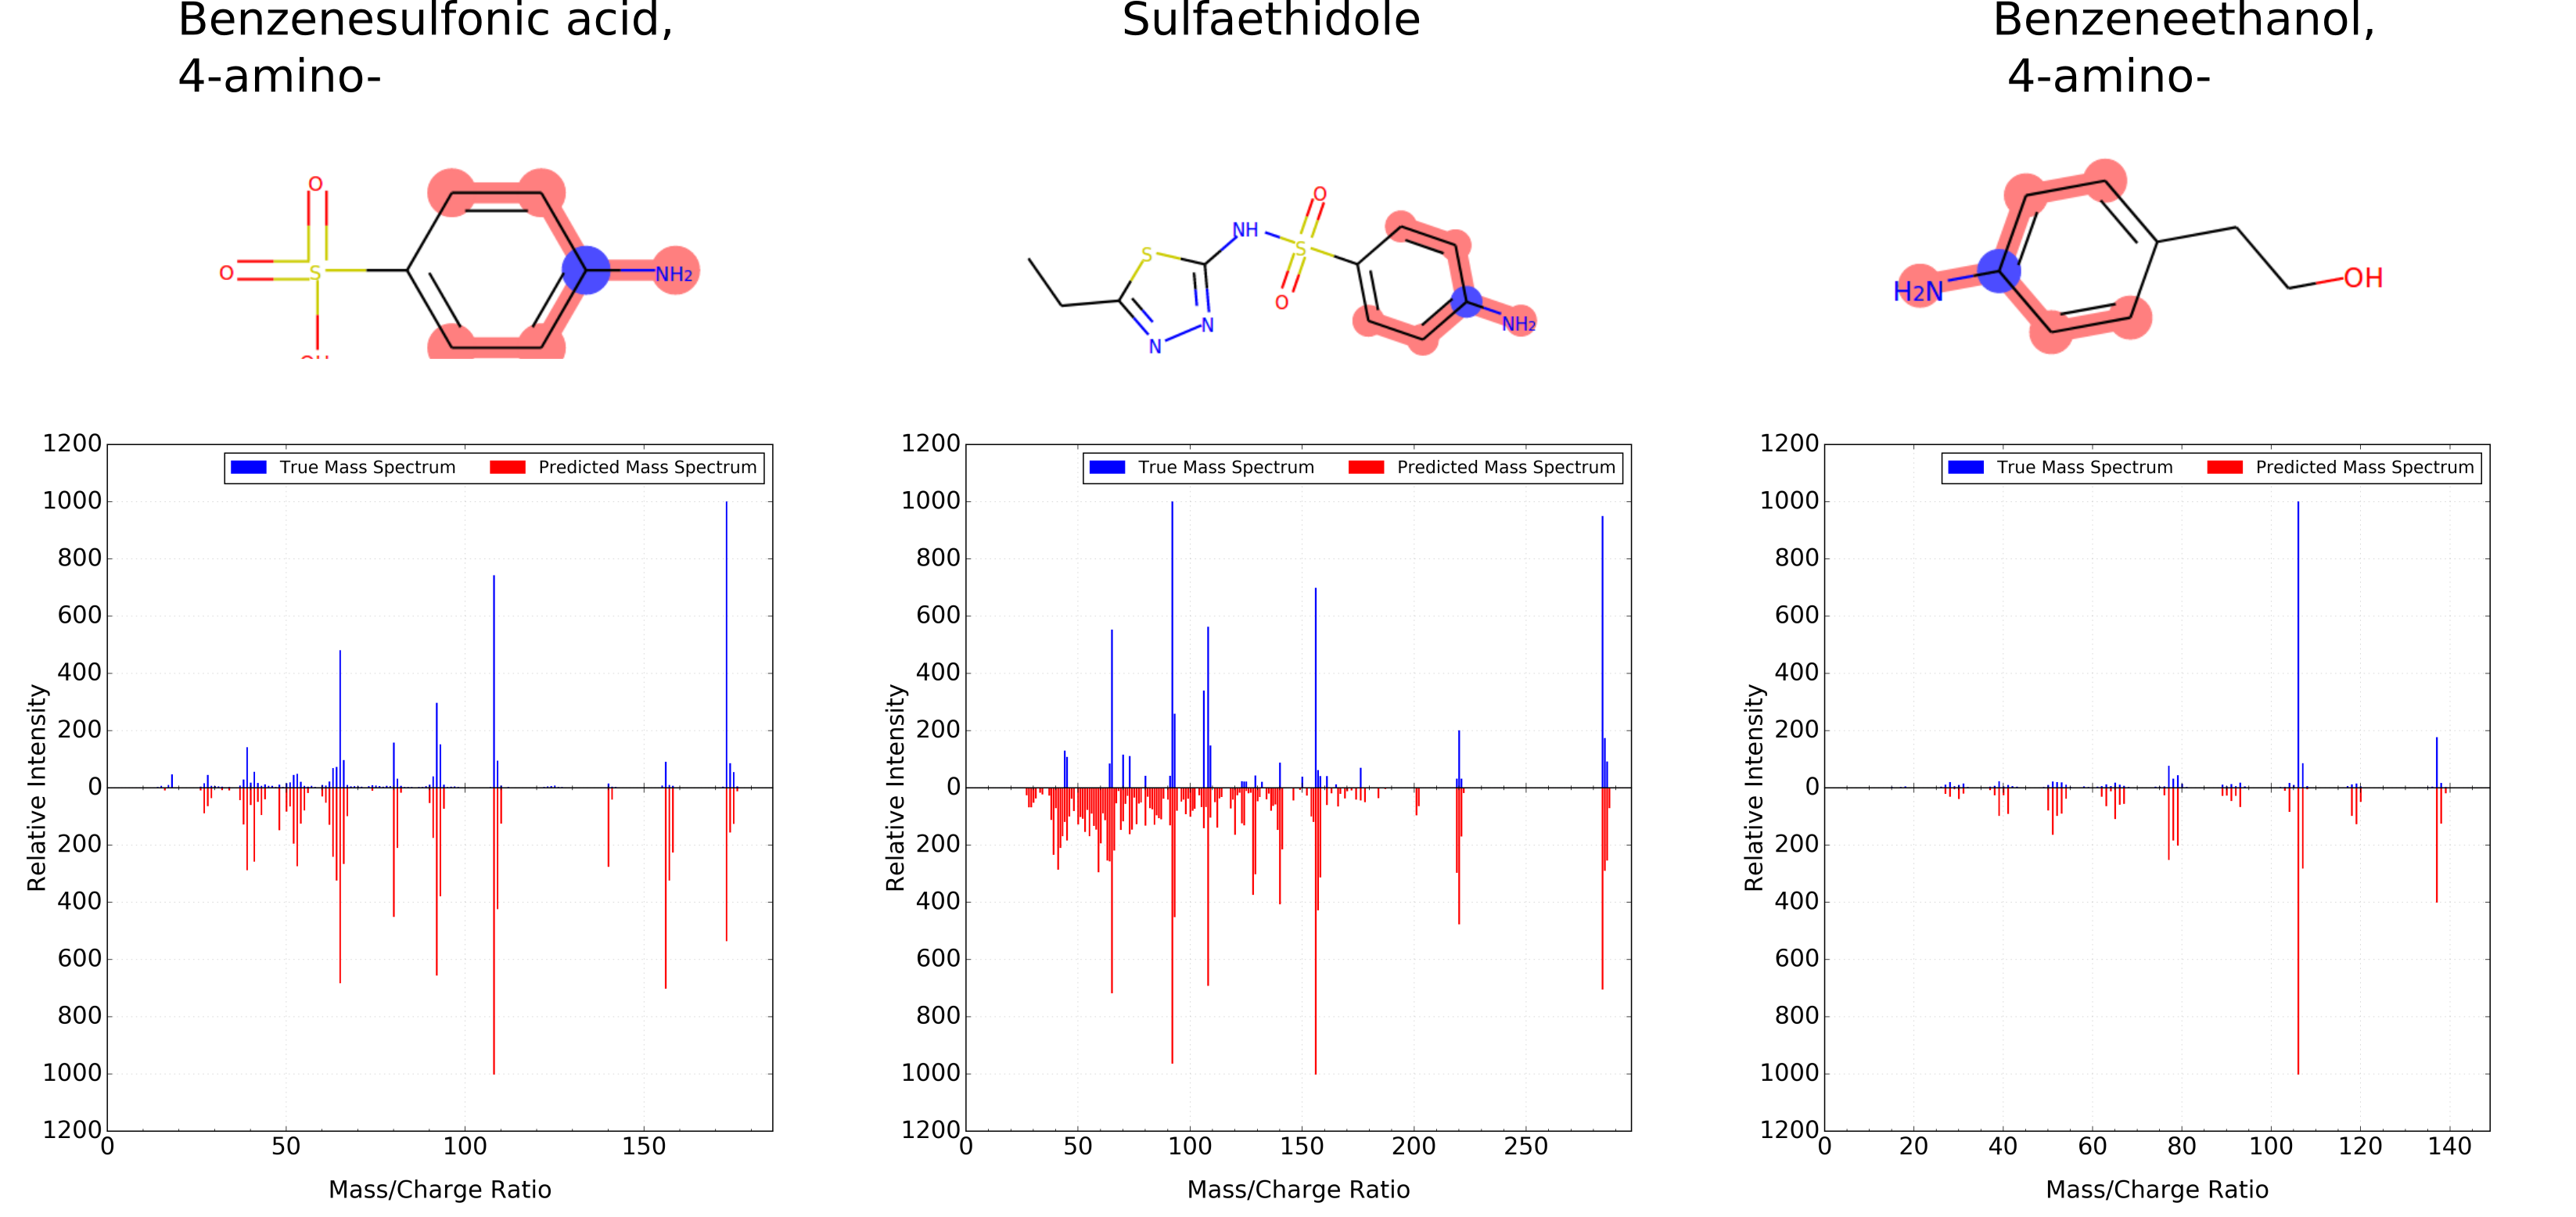
\includegraphics[width=0.95\linewidth]{bit_3852_highlight_spectra_2.png}
        \caption[Spectral Prediction Examples for bit 3852]{Spectral predictions for some molecules containing bit 3852. Note the presence of a peak at \textit{m/z} = 93. This peak corresponds to the presence of the aniline ion. This peak is predicted even for the third molecule, where there is no peak at 93 in the ground truth spectra.}
    \label{fig:bit_example_spectra}
\end{figure}

We explore the predictions for bit 3852, one of the high performing bits, in Figure\ref{fig:bit_example_spectra}. Bit 3852 typically corresponds to the aniline fragment (highlighted on the top molecule) as shown. Due to its stability, molecules containing an aniline functional group often ionize to leave an anilium ion, whose mass is 93Da. Peaks at 93 can be observed observed in the predicted spectra for all 3 molecules.

\section{Conclusion}

We demonstrate that NEIMS achieves high library matching performance on an augmented spectral library containing predictions for molecules in the query set. 
The performance of NEIMS is slightly better than existing machine learning models for predicting EI-MS spectra, with significant boost in speed of prediction.

The high performance in library matching is attributable to the bidirectional prediction mode which allows the model to more accurately to predict intensities for fragments corresponding to the molecular mass less the mass of a common subgroup. We observe that the improvement in the library matching task also corresponds with improvement in similarity of the predicted spectra to the ground truth. We also observe a case study of the spectra of some molecules containing the same subgroup.

Several adjustments could be made to further improve NEIMS. For example, NEIMS currently does not have a method to model intensity peaks corresponding to ion fragments containing isotopes. If we were to train on spectral data with greater precision in the peaks locations, we might be able to train our model to learn the exact identities of the atoms based on the decimal values of the \textit{m/z} peak locations.

Furthermore, different molecular representation could be tested. The predictions made from ECFP are limited by the descriptiveness of the fingerprint~\cite{rdkit_blogpost_collide_bits}. In particular, the overlap in representation for different molecular features represents a huge limitation to the representation of the molecule. Additionally, ECFPs are not equipped to predict to represent molecules with different chiralities, which will have different spectra, so a descriptor that incorporates 3D geometries may be useful. It would also be interesting to explore whether a bond-based molecular fingerprint representation\cite{kearnes2016molecular} may improve performance.

The lightweight framework of NEIMS makes it possible to rapidly generate spectral predictions for large numbers of molecular candidates. This collection of predicted spectra can then be used directly in mass spectrometry software to expand the coverage of molecules which can be identified by mass spectrometry. Because the requirements of NEIMS has limited dependence to EI mass spectrometry, it likely that some of the principles used here could be extended to electrospray ionization mass spectrometry.

\section{Acknowledgments}
We thank Stephen Stein for providing access to the SDF versions of the NIST 2017 and NIST 2014 Mass Spectral Libraries, and for his useful insights. We thank Laura Castellanos for her insights and comments about the paper. We thank Steven Kearnes for the internal review, and Lucy Colwell and Michael Brenner for their enlightening conversations.
